\documentclass[margin=3mm]{standalone}
\usepackage{tikz}
\usetikzlibrary{arrows.meta,
                positioning,
                quotes,
                shadows.blur}

\begin{document}
    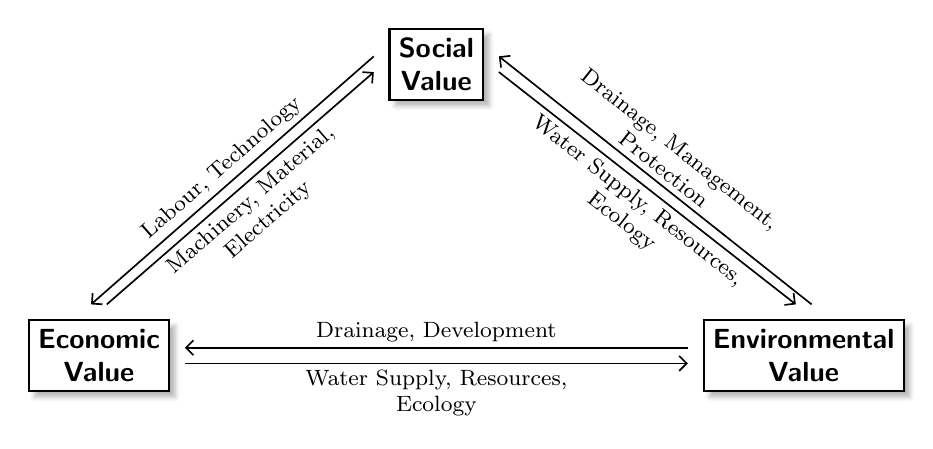
\begin{tikzpicture}[
node distance = 24mm and 24mm,
     N/.style = {draw, thick, font=\sffamily\bfseries, align=center,
                 fill=white, outer sep=2mm, blur shadow={shadow opacity=30}},
every edge/.style = {draw, -Straight Barb, semithick},
every edge quotes/.append style = {auto, font=\footnotesize, inner sep=2pt, align=center, sloped}
                        ]
% Nodes
\node (n1) [N]  {Social\\ Value};
\node (n2) [N, below  left=of n1]   {Economic \\ Value};
\node (n3) [N, below right=of n1]   {Environmental \\ Value};
% Arrows
\draw   ([yshift= 1mm] n1.west)  edge["{Labour, Technology}"]                   ([xshift=-1mm] n2.north)
        ([xshift= 1mm] n3.north) edge["{Drainage, Management,\\ Protection}"]     ([yshift= 1mm] n1.east)
        ([yshift=-1mm] n2.east)  edge["{Water Supply, Resources,\\ Ecology}" ']   ([yshift=-1mm] n3.west);
\draw   ([xshift= 1mm] n2.north) edge["{Machinery, Material,\\ Electricity}" ']   ([yshift=-1mm] n1.west)
        ([yshift= 1mm] n3.west)  edge["{Drainage, Development}"]     ([yshift= 1mm] n2.east)
        ([yshift=-1mm] n1.east)  edge["{Water Supply, Resources,\\ Ecology}" ']                 ([xshift=-1mm] n3.north);
    \end{tikzpicture}
 \end{document}